\documentclass{report}

\usepackage{graphicx}
\usepackage[utf8]{inputenc}
\usepackage{hyperref}
\usepackage{fancyvrb}
\usepackage[dvipsnames]{xcolor}
\usepackage[spanish]{babel}
\usepackage[numbers]{natbib}

\hypersetup{
	colorlinks,
	citecolor=black,
	filecolor=black,
	linkcolor=blue,
	urlcolor=black
}

% redefine \VerbatimInput
\RecustomVerbatimCommand{\VerbatimInput}{VerbatimInput}%
{
	fontsize=\footnotesize,
	%
	frame=lines,  % top and bottom rule only
	framesep=2em, % separation between frame and text
	rulecolor=\color{Gray},
	%
	% label=\fbox{\color{Black}data.txt},
	% labelposition=topline,
	%
}

\author{Ezequiel Santamaría Navarro}
\title{Trabajo fin de grado sobre la construcción de un entorno de aprendizaje pre-universitario para la programación.}


%\renewcommand{\abstractname}{Abstracto}
%\renewcommand{\contentsname}{Índice de contenido}
\renewcommand{\chaptername}{Parte}

\begin{document}
	\maketitle
	\tableofcontents
	
	\begin{abstract}
		Proceso de creación de un lenguaje sencillo, de un entorno de programación sin instalación y con herramientas para facilitar el desarrollo.
	\end{abstract}
	
	
	\chapter{Introducción}
	
	%TODO: Añadir una introducción
	
	\section{Objetivo e intenciones de este trabajo}
	
	%TODO: Formalizar esto
	
	La enseñanza preuniversitaria de la programación consiste en enseñar a adolescentes y niños a poder pensar de forma lógica y abstracta. Esto conlleva un conjunto de problemas distintos al de la enseñanza a nivel universitario. Antes de la universidad no se puede asumir si los alumnos conocen o no ciertas partes de las matemáticas, si saben o no dibujo técnico, o incluso si entienden como funciona un espacio de coordenadas cartesianas.
	
	En mi caso concreto, la primera vez que empecé con un lenguaje de programación (uno que se use de forma profesional) fue Pascal con Delphi (en 2007). Fue mi hermano mayor quien me ayudó a instalar tanto el IDE como quien me explicó algunas directrices para empezar a hacer aplicaciones muy básicas.
	
	Durante dos años intenté hacer dos cosas muy concretas con Delphi que no conseguí y que me causaron frustración: dibujar (como en un lienzo, algunos gráficos) y conectar la aplicación a internet con otra copia de la aplicación.
	
	La sensación que he tenido desde entonces hasta hoy es que los lenguajes de programación están orientados a ser útiles desde la perspectiva de un ingeniero, pero no de facilitar el aprendizaje. 
	
	Por ello, mi objetivo sería conseguir que el proyecto cumpla los siguientes puntos:
	
	\begin{itemize}
		\item El lenguaje debe estar en la medida de lo posible en castellano, para no asumir que el alumno entiende inglés.
		\item El lenguaje preferiblemente será tiapdo, con comprobación de tipos \cite{statictypecheck}\cite{typesafety} y sin operaciones de memoria \cite{memorysafety} (como los punteros de C o C++, que permiten el bypass de tipos). 
		\item El lenguaje tendrá tipos de datos con nombres comunes. Por ejemplo, se evitará el uso de Mapa y Vector, y se usarán nombres como Relación y Lista respectivamente.
		\item No debe asumir automáticamente conversiones de datos. Bajo mi perspectiva, el alumno debe ser consciente de que los datos tienen un representación que se puede convertir, pero que el ordenador no es inteligente y hay que dar órdenes explícitas.
		\item Que no requiera instalador, importantísimo para evitar frustraciones con el software. 
		\item Si fuera posible, integrable con la herramienta Descubre, para aprovechar el sistema de usuarios y de compartir los ejemplos que ya tiene.
		\item Que sea flexible para que los docentes puedan añadir funcionalidad, ampliando el conjunto de problemas, ejemplos, soluciones y aplicaciones.
	\end{itemize} 
	
	Estos son los puntos fundamentales que podrían simplificar el aprendizaje del desarrollo algorítmico y la programación.
	
	\section{Ideas extraídas de los distintos proyectos}
	
	Las ideas que más me han gustado y que desarrollo en el siguiente capítulo son:
	
	\begin{itemize}
		\item Editor y ejecución (compilación transparente) en una misma web como Descubre o CodeCombat.
		\item Un lenguaje propio simplificado como iJava. 
		\item Mezcla de imperativo y con objetos (aunque mayoritariamente imperativo) con una lista de subrutinas para dibujar como Processing.
		\item Intentar advertir de los errores de compilación con lenguaje sencillo evitando tecnicismos si es posible, como con el editor de Khan Academy
		\item Ofrecer un editor que ayude al alumno a escribir el código, sugiriendo nombres, autocompletando según el contexto...
	\end{itemize}
	
	\chapter{Estado del arte}
	
	\section{Entornos de aprendizaje a la programación}
	
	Investigando proyectos con puntos comunes a lo que busco, estos son los proyectos que he podido ver y me han sorprendido en algún o varios aspectos. Existen muchos más, pero estos ofrecen en conjunto lo mismo (o lo más destacable) que el resto.
	
	\subsection{Descubre}
	
	La herramienta Descubre, desarrollada por Juan Antonio Sánchez Laguna, Marcos Menárguez Tortosa, y Juan Antonio Martínez Navarro. 
	
	La herramienta se compone de:
	
	%TODO meter bibliografía y referencias de processing.
	
	\begin{itemize}
		\item Un editor de texto, derivado de CodeMirror.
		\item Un lenguaje de programación propio, derivado de Java, con un las funcionalidades de processing.
		\item Un entorno con un lienzo para dibujar y una salida para escribir texto.
		\item Un repositorio de usuarios y programas que permite copiar el código de otros para hacer clones. 
	\end{itemize}
	
	Con los siguientes puntos positivos:
	
	\begin{itemize}
		\item Entorno completo. Desde escribir el código hasta ver su resultado en la misma página.
		\item Sin instalación y sin necesidad de conocimientos sobre compilaciones.
		\item El lenguaje comparte sintaxis con C y Java, lo que es útil para avanzar más allá de la enseñanza. 
		\item La página tiene una lista de tutoriales y documentación sobre la funcionalidad de processing.
		\item Se puede clonar con facilidad el código de otros alumnos o docentes.
	\end{itemize}
	
	Y los siguientes puntos negativos:
	
	\begin{itemize}
		\item El lienzo es un poco pequeño. Se limita a 320x320. Tiene una versión estirada del mismo que se ve pixelada, y otros sistemas (como por ejemplo, \hyperref[app:b]{codecombat, Apéndice B})
		\item La sintaxis de iJava no es amigable para nuevos alumnos.
		\item La ejecución del código es síncrono. Esto reduce las posibilidades tecnológicas. Como por ejemplo, no se pueden cargar imágenes en tiempo de ejecución.
		\item No se puede rotar el lienzo, así que todos los dibujos deben estar alineados a los ejes de coordenadas.
		\item No se puede extender el lenguaje con el propio lenguaje. Es decir, no se puede escribir un módulo para que se incluya en otro código. Esta parte no es importante para el alumno, pero sí para el docente que quiera extender el lenguaje.
	\end{itemize}
	
	\hfill
	
	Acceso: \url{http://descubre.inf.um.es}
	
	\subsection{Codecombat}
	
	CodeCombat es un proyecto de código abierto para aprender a programar en base a un juego multijugador. Actualmente tiene varios problemas sencillos (que van creciendo en dificultad) para ir aprendiendo los mecanismos de los distintos lenguajes que ofrece, a la vez que vas ganando monedas para poder comprar objetos que ofrecen mayor funcionalidad (te permiten usar más métodos para resolver los distintos problemas).
	\\
	
	Se pueden destacar los siguientes puntos del proyecto:
	
	\begin{itemize}
		\item Gran conjunto de problemas a resolver que van creciendo en dificultad.
		\item Permite seleccionar entre Python, JavaScript, Clojure, CoffeScript y Lua.
		\item Acabado artístico profesional, así como una gran cantidad de objetos.
		\item Proyecto de código abierto.
		\item Traducido (parcialmente) a varios idiomas, entre los cuales se encuentra el español.
	\end{itemize}
	
	Sin embargo, el objetivo de esta plataforma es aprender resolviendo problemas concretos como moverse por un laberinto, o eliminando unos enemigos, pero no crear otras aplicaciones. Aún así, es una muy buena herramienta de aprendizaje.
	
	Como punto negativo destacaría que te obligan a programar en un lenguaje real, sin ofrecerte una alternativa amigable para nuevos alumnos. Que por defecto, Python, tiene problemas con la indentación obligatoria, que podría ser una barrera.
	
	Se puede probar sin registro. Hay una imagen de ejemplo de la aplicación en el \hyperref[app:b]{apéndice B de CodeCombat}.
	
	\hfill
	
	Acceso: \url{http://codecombat.com}
	
	\subsection{Scratch}
	
	Scracth es un proyecto impulsado por el MIT para el desarrollo de pequeños proyectos con dibujos, animaciones y sonidos. 
	
	Se basa en programar unos módulos encajando unas piezas que equivalen a sentencias, instrucciones o elementos de control en un lenguaje
	por bloques, como si fuera un juego de Lego en dos dimensiones.
	
	El lenguaje y el editor tienen versión web y versión local, que se encuentra en paquetes como la Raspberry Pi. En la versión web, se pueden alojar proyectos para que 
	sean de dominio público y cualquier persona puede clonarlo para alterarlo a su gusto.
	
	De este proyecto cabe destacar la gran cantidad de usuarios, así como la interfaz y la posibilidad de no necesitar la web para hacer un proyecto. Además, los bloques que conforman el código están traducidos a varios idiomas, reduciendo la barrera de los alumnos que aprenden en castellano.
	
	La única pega que le veo al proyecto es que la programación es por bloques, y que la interfaz, en mi opinión, está enfocado a alumnos muy jóvenes (de edades entre 6 y 12 años). 
	
	\hfill
	
	Acceso: \url{https://scratch.mit.edu}
	
	\subsection{code.org}
	
	Code.org es una web con varios tipos niveles de problemas, donde hay un lienzo representando un problema. Los alumnos (recomendado de 4 a 18 años) resuelven unos problemas que crecen progresivamente en dificultad. A diferencia de codecombat, code.org utiliza un lenguaje basado en bloques como el de Scratch. 
	
	Los problemas son visualmente muy entretenidos (como los de codecombat), aunque más enfocados a alumnos más jóvenes (desde 4 años).
	
	Al igual que Scratch, esta web ofrece los bloques de código en castellano, y unos vídeos introductorios interesantes con subtítulos al español.
	
	La pega que le veo es la misma que a Scratch y Codecombat: solo ofrecen un mecanismo para resolver problemas, con una interfaz basada en bloques y con una temática enfocada a niños pequeños.
	
	\hfill
	
	Acceso: \url{http://code.org}
	
	\subsection{Khan Academy - Aprendiendo a dibujar con Javascript}
	
	En Khan Academy hay un conjunto de tutoriales para aprender JavaScript con el objetivo de dibujar en un lienzo como el de Descubre. Tiene muchos tutoriales y son todos interactivos y subtitulados al castellano.
	
	\hfill
	
	De aquí cabe destacar que el editor es muy interactivo. Permite la edición de casi cualquier valor con una especie de elemento visual. Además, el código se compila automáticamente (en el caso de javascript se podría evaluar directamente) y se pinta en el lienzo cada vez que el código cambia. 
	
	\hfill
	
	Acceso: 
	\href{https://es.khanacademy.org/computing/hour-of-code/hour-of-code-tutorial/p/intro-to-drawing}{Intro to Drawing}
	
	\section{Compiladores y analizadores escritos en javascript}
	
	\subsection{Jison - Bison para javascript}
	
	Jison es un proyecto escrito en Javascript que ofrece las herramientas similares a GNU Bison, un analizador de gramáticas libres de contexto de tipo LALR(1) \cite{bison}.
	
	Según mis cálculos (indicados más adelante) en el apartado \textit{Definición del lenguaje ZL} es necesario al menos un analizador que avance 3 tokens antes de conocer la derivación a realizar. Así que descarto Jison ya que no creo que sea suficientemente potente para analizar ZL. 
	
	Acceso:
	\href{https://github.com/zaach/jison}{Github de jison}	
	
	\subsection{Analizador descendente recursivo por prioridad de operadores}
	
	El analizador descendente (Top Down) por orden de prioridad de operadores (Operator Precedence) fue presentado por Vaughan Pratt en el año 73 \cite{acmtdop}. El analizador se basa en definir unos símbolos, unas expresiones y unos operadores (indicando su prioridad de forma numérica) con funciones recursivas que indican el comportamiento a la hora de ir avanzando recursivamente.
	
	
	En principio mi plan era utilizar este analizador como LL(3), pero mientras avanzaba con la implementación del análisis, ceñirse estrictamente al uso de este analizador era cada vez más difícil. 
	
	Sin embargo, este tipo de análisis ha inspirado la forma en la que he escrito el analizador sintáctico, usando reglas de derivación de forma recursiva donde en cada una de ellas se indica
	cómo se debe avanzar y cuál es el resultado generado. 
	
	Acceso:
	\href{http://javascript.crockford.com/tdop/tdop.html}{Texto de Douglas Crockford}
	
	\subsection{Analizador de gramáticas de expresiones}
	
	%TODO: http://pegjs.org/online
	%TODO: https://en.wikipedia.org/wiki/Parsing_expression_grammar
	
	\section{Editores de texto para Javascript y HTML}
	
	Lo primero que he encontrado ha sido el editor Codemirror. Es el mismo editor que usa el proyecto Descubre de la facultad. No me he dedicado en buscar otros editores porque este tiene
	todo lo que necesito para poder preparar el entorno, y además su API está muy bien documentada\cite{codemirrorapi}.
	
	Acceso:
	\href{http://codemirror.net/}{Página web oficial de codemirror.}
	
	\chapter{Análisis de objetivos y metodología}
	
	Los objetivos principales han sido crear un lenguaje con palabras cercanas al lenguaje común español, un editor de texto amigable y un compilador de dicho lenguaje, buscando en la medida de lo posible el respaldo de unos usuarios a los que medía su grado de entedimiento.
	
	\vspace{10px}
	
	He empleado una metodología que he separado en tres pasos: investigación, implementación y feedback. Con esos tres pasos he hecho varias iteraciones. En esta sección resumo la implenetación ya que más adelante se habla en detalle de las implementaciones.
	
	\vspace{10px}
	
	El primer objetivo era definir el lenguaje. Aunque ha ido cambiando a lo largo de todo el proyecto, gran parte de lo definido al principio no ha cambiado. Aquí la investigación ha sido básicamente encontrar una forma de definir el lenguaje, en el cual me acabé decantando por la forma de BNF\cite{bnf} con alguna modificación, aunque también estudié la posibilidad de usar DCG\cite{dcg} pero la descarté por parecer más compleja de entender. 
	
	La implementación ha sido sencillamente escribir la sintaxis en formato BNF (\hyperref[app:a]{en el apéndice A o el fichero sintaxis.txt}), y el feedback ha sido preguntar a los usuarios sobre que estructuras y palabras les han parecido más sencillas de comprender dando a elegir entre varias opciones (las constantes booleanas verdadero/falso o cierto/falso o verdadero/mentira, entre otras).
	
	\vspace{10px}
	
	El segundo objetivo es escribir el compilador, pero para ello necesito un editor para poder ir haciendo las pruebas, así que como objetivo intermedio se hace el editor. La investigación aquí es corta: ya conozco codemirror y además se usa en Descubre para iJava, sé que ofrece un plugin sencillo para colorear texto\cite{codemirrorsyntaxhighlight} y un plugin para autocompletar \cite{codemirrorautocomplete}. 
	
	La implementación para este objetivo es relativamente sencilla, y se divide entre los ficheros \textbf{index.html} (se instancia el editor), \textbf{autocompletar.js} (se definen las órdenes de autocompletado) y \textbf{editor.js} (se definen las órdenes de coloreado de sintaxis). Aquí el feedback que he podido obtener de los usuarios ha sido relativo a la facilidad de lectura del texto y a la facilidad del autocompletado, habiendo cambiado el algoritmo de autocompletado gracias a las indicaciones de los usuarios (de un algoritmo LCS a uno que use distancias de Levensthein). 
	
	Una vez definido lenguaje y editor, falta el último objetivo, el más complejo y quizá el más importante: el compilador. Al principio, al ver las distintas alternativas de analizadores escritos en Javascript opté por usar pegjs (en la siguiente sección se explica con más detalle), pero al final he escrito mi propio analizador. La diferencia entre escribir mi propio analizador y usar otro tampoco es tan grande ya que después de analizar la gramática libre de contexto hay que generar una tabla de símbolos, hacer comprobaciones semánticas y luego transformar a Javascript, que es la parte más compleja con diferencia.
	
	El compilador se separa en varios ficheros, pero como son muchos entraré en más detalle sobre la implementación en la sección de la estructura del compilador para ZL. De aquí no puedo obtener mucho feedback salvo la generación de errores si el código escrito no pasa alguna de las fases de compilación, para ver si los usuarios son capaces de entender los errores y corregirlos.
	
	\section{Desarrollo de un entorno de programación}
	Al igual que Descubre o Codecombat, el principal objetivo del trabajo es crear un entorno para facilitar la programación. Este sistema debe estar compuesto de al menos un editor de texto, el compilador del lenguaje diseñado y las herramientas de entrada y salida (barras de texto para escribir, lienzos para dibujar, eventos de teclado...). Recomendablemente el entorno debe tener información sobre depuración (errores al escribir el código, información de depuración al pausar el código, etc...) como tienen también otros entornos (Descubre o Codecombat, por ejemplo).
	
	
	\subsection{Compilador del lenguaje ZL}
	En una primera aproximación el compilador se construyó usando PEG.js\cite{pegjs}, que en su descripción dice ser más potente que LL(k) o LR(k). Sin embargo, no fui capaz de hacer análisis de un trozo ambiguo de ZL. El problema lo localicé al intentar analizar el siguiente trozo de pseudo-ZL (en los inicios, la sintaxis era mucho más sencilla):
	
	\begin{BVerbatim}
	x es Booleano
	x <- falso
	Si no x hacer // if (!x)
		mostrar [
			mensaje <- "x es falso"
		]
	si no hacer // else
		mostrar [
			mensaje <- "x es verdadero"
		]
	fin
	\end{BVerbatim}
	\\
	
	Aquí localicé tres problemas de los cuales supe resolver 2. El primero es diferenciar `si no \textbf{x}' de `si no \textbf{hacer}'. Se resuelve fácilmente diferenciando gramaticalmente un nombre (por ejemplo, `x') de ciertas palabras reservadas como `hacer'. Con esto se fuerza un error si el analizador se encuentra con `si' e intenta reducir/derivar `no hacer' como una expresión, ya que para que fuese una expresión `hacer' no debería ser una palabra reservada, sino un nombre.
	
	\vspace{10px}
	
	El segundo problema es, precisamente, evitar el uso de la palabra \textbf{hacer} como nombre, pero se resuelve fácilmente usando expresiones regulares negativas (\hyperref[app:c]{Javascript permite lo que se llama} negative lookahead\cite{lookahead}). 
	
	\vspace{10px}
	
	El tercer problema, que no he sido capaz de resolver usando PEG.js, viene a ser que, si se escribe mal el código del segundo si condicional, el compilador advierte de que no se pudo resolver el primer si condicional. Por ejemplo, si en vez de escribir `si no hacer' se escribiera `si mo hacer' el compilador indicaría error en el primer si condicional, debido a que si no se puede reducir correctamente el segundo si no hacer, lo intenta analizar después como un si condicional, pero como `mo hacer' no es una expresión correcta, no se puede reducir/derivar el primer si condicional, dejando ahí marcado el error.
	
	\vspace{10px}
	
	Viendo la serie de problemas que tenía con gramáticas sencillas pero ambiguas, lo único que quedaba era o alterar los compiladores ya escritos o implementar uno por cuenta propia. Uno que ofrezca los mismos mecanismos que los otros compiladores pero que me permita romper el comportamiento por defecto (que admita cierta flexibilidad) para añadir información de error, o para resolver el problema de los múltiples si condicionales. Al final me decanté por la segunda opción, con la esperanza de que llevase menos tiempo que alterar PEG.js.
	
	\subsection{Editor de texto inteligente}
	
	Los puntos planteados para hacer el editor inteligente pasan básicamente por dotar a un editor la capacidad de autocompletar. El lenguaje es verboso y los datos son tipados, haciendo posible la inferencia desde el editor de las posibles y diferentes compleciones. Como se ve en la siguiente sección (Definición del lenguaje ZL), la asociación de argumentos de subrutinas es por nombre. Esto hace que el lenguaje sea más fácil de leer sin memorizar, aunque más difícil de escribir:
	
	\vspace{10px}
	
	\begin{BVerbatim}
	En iJava, por ejemplo:
	ellipse(100, 200, 50, 50);
	\end{BVerbatim}
	
	\vspace{10px}
	
	\begin{BVerbatim}
	En ZL:
	elipse [
		centro <- {100, 200} como punto
		ancho <- 50
		alto <- 50
	]
	\end{BVerbatim}
	
	Para reducir la dificultad a la hora de escribir\footnote{La parte del código que pone `como punto' es un conversor que indica que \{100, 200\} es un punto bidimensional.}, es importante un buen editor que ayude a autocompletar, sugiriendo nombres y escribiendo los distintos argumentos de las subrutinas, como por ejemplo:
	
	
	\begin{center}
	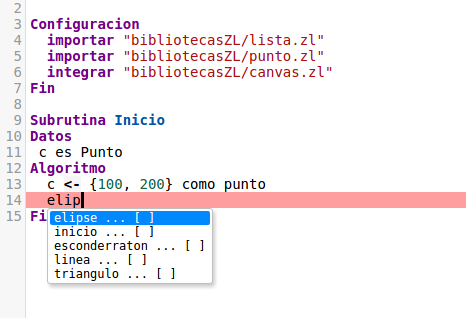
\includegraphics[width=0.4\linewidth]{beforecompletion}
	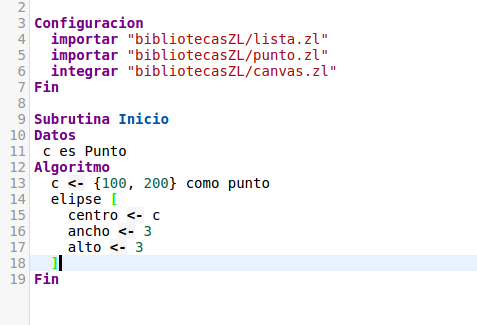
\includegraphics[width=0.4\linewidth]{aftercompletion}
	
	A izquierda, el menú contextual que aparece al escribir `elip'. A la derecha, lo que aparece \textbf{inmediatamente después} de pulsar \textit{enter} o seleccionar con el ratón. `Ancho'  y `alto' se autocompletan con un número por defecto (3 es el número por defecto elegido arbitrariamente), y centro se autocompleta con el dato `c', inferido a través de los tipos de los datos.   
	\end{center}
	
	El funcionamiento y la implementación del autocompletado se ve más adelante en la sección \textbf{Editor inteligente - Autocompletado}.
	
	\section{Definición del lenguaje ZL}
	
	A la hora de definir el lenguaje ZL me centré en varios aspectos que tomé como fundamentales: que fuese cercano al lenguaje natural, y que estuviese en español\cite{mundoingles}.
	
	\vspace{10px}
	
	Parte del léxico usado para definir el lenguaje está escogido en base a probar a personas con diferentes formaciones: sin formación informática, con nociones pero sin conocimiento de programación, ex-programadores... Las pruebas han sido, básicamente, medir su grado de entendimiento de las estructuras del lenguaje con diferentes formas. 
	
	\vspace{10px}
	
	Los nombres escogidos se acercan más al lenguaje cotidiano que al lenguaje informático. Se ha preferido nombres como `Lista' y `Relacion' frente a `Vector' o `Mapa'. Se ha escogido el nombre `Dato' frente a `Variable'. Se usan palabras para abrir y cerrar bloques como `Hacer' y `Fin' en vez de llaves \{\}. 
	
	\vspace{10px}
	
	Por haber elegido la construcción de un lenguaje cercano al lenguaje natural aparecen repeticiones, sobretodo por usar las mismas palabras reservadas en contextos distintos: `si' para indicar el equivalente a `if' o `else' (en C), `no' para indicar negación de verdad o `else'... Esto causa que el lenguaje sea LL(3) (para ver el lenguaje en formato BNF extendido, \hyperref[app:a]{ver apendice A}) en la siguiente regla de derivación:

	\vspace{10px}
	
	\begin{verbatim}
	<sicondicional> ::= "si" <_> <expresion> <_> "hacer" <_> (<sentencia> <_>)+ "fin"
	| "si" <_> <expresion> <_> "hacer" <_> (<sentencia> <_>)+ <sinocondicional>
	| "si" <_> <expresion> <_> "hacer" <_> (<sentencia> <_>)+ <sino>
	\end{verbatim}
	
	A simple vista se puede ver como es LL(2), al empezar todas las reglas con "si". Después de factorizar el "si", es donde viene el problema. La primera regla es un `if' (de C) seguido de ningún `else' y ningún `else if'. La segunda regla, de un `if' seguido de al menos un `else if'. La tercera regla, un `if' acabado de un `else'. El problema viene con la tercera regla, ya que:
	
	\vspace{10px}
	
	\begin{BVerbatim}
<sino> ::= "si" <_> "no" <_> "hacer" <_> (<sentencia> <_>)+ "fin"

// Ejemplo de código de conflicto LL(3)
Si x hacer
	Si no y hacer
		// ...
	Fin
Si no hacer
	// ...
Fin
	\end{BVerbatim}
	
	\vspace{10px}
	
	El conflicto\cite{conflictoll3} viene que hasta que no se lee `Si no \{siguiente token\}' no se puede distinguir entre un `if' anidado dentro de otro `if' (Si no y hacer) y un `else' (Si no hacer).
	
	\subsection{Descripción de la notación BNF ampliada}
	
	La notación BNF que utilizo en el \hyperref[app:a]{Apéndice A} es una notación BNF a la cual he añadido paréntesis para agrupar, y los operadores *, + y ? como operadores de repetición. Funcionan como en las expresiones regulares: * para indicar cero o más veces, + para indicar uno o más veces, y ? para indicar cero o una veces. 
	
	Los siguientes ejemplos son equivalentes en BNF:
	
	\begin{BVerbatim}
BNF extendido:
a ::= b c?
x ::= (y z)*
j ::= k (l m)+

BNF:
a ::= b
    | b c
j_plus ::= l m
    | j_plus l m	
j ::= k j_plus
x ::= 
    | y z x
	\end{BVerbatim}
	
	\subsection{Gramática BNF del lenguaje}
	% TODO: Cambiar por una descripción menos formal
	La gramática del lenguaje en formato BNF se puede ver en el \hyperref[app:a]{Apéndice A}. De ella, cabe destacar de la gramática las 4 expresiones y los cuatro grupos de operadores, para poder definir correctamente el orden en el cuál los operadores se reducen. En la implementación no uso esa técnica para definir el orden de las operaciones, sino que una vez construido el árbol de la expresión, cambio sus ramas para que respeten el orden de los operadores. 
		
	\vspace{10px}
		
	Otros conceptos destacables en la gramática es el uso de diferentes tipos de enumerar (en hexadecimal, decimal, o binario). 
	
	\subsection{Descripción de la semántica}
	
	Las estructuras semánticas del lenguaje se puede clasificar en módulos, subrutinas, algoritmos, datos y configuraciones. Parte de la semántica es compleja y está enfocada para los posibles docentes y para usuarios avanzados. Los alumnos nuevos que quieran aprender pueden centrarse en escribir solo algunas subrutinas e ignorar todo el resto de las estructuras.
	
	\vspace{10px}
	
	Para darle flexibilidad al lenguaje, el lenguaje está pensado para escribirse en módulos. Los módulos se pueden ver como unidades de código que se pueden compilar, y a su vez los módulos pueden incluir otros módulos. Un módulo puede tener configuraciones, y puede tener subrutinas. 
	
	\vspace{10px}
	
	Las subrutinas son la estructura básica de ejecución. En una subrutina se define un algoritmo, que indica el comportamiento de la subrutina, así como los datos que el algoritmo va a usar. A su vez, la subrutina puede tener modificadores que alteran el comportamiento del código sobre la subrutina. Por ejemplo, el modificador \textbf{subrutina primitiva} permite ejecutar código nativo javascript en una subrutina (ver más adelante la sección Código nativo), que está definida en ZL.
	
	\vspace{10px}
	
	Los datos, dentro de una subrutina, se definen por un nombre, un tipo, y un ámbito: local, de entrada, de salida, de entrada y salida, o global. Cuando un dato es de tipo local, solo la subrutina que lo define conoce su valor y puede acceder a él. Los datos de ámbito de entrada se proporcionan al llamar a la subrutina, y no se pueden escribir sobre ellos. Los datos de ámbito de salida se deben proporcionar en la subrutina y son leídos (opcionalmente) al llamar a la subrutina. Los datos de tipo global tienen ámbito \textbf{dentro de un módulo}. Todas las subrutinas que definan el mismo dato (que debe, por obligación de compilación, coincidir en tipo y nombre) podrán compartir el valor, y estos datos deben inicializarse en la \textbf{subrutina inicio} de cada módulo (cada módulo inicializará sus datos globales), usándose esa subrutina como constructor. 
	
	\vspace{10px}
	
	Una configuración define constantes que pueden ser útiles para el entorno (como por ejemplo, el número de fotogramas por segundo, cuántos decimales se imprimen por defecto, el ancho y el alto del lienzo...), además de permitir incluir módulos de dos formas distintas: \textbf{integrar} o \textbf{importar}. \textbf{Integrar} un módulo equivaldría a un `\#include' de C o C++, donde el código se `copia y pega' en el lugar de la directiva. Las subrutinas del módulo integrado forman parte del entorno del módulo que lo integra. Por otra parte, \textbf{importar} un módulo equivale a un `import' de Java. Se crea un nuevo tipo de dato (una clase si hablamos en términos Java) cuyas subrutinas pasan a ser parte de ese tipo (como si fuesen miembros, en Java).
	
	\vspace{10px}
	
		
	\chapter{Diseño y resolución del trabajo realizado}
	
	\section{Estructura del compilador para ZL}
	
	%TODO: Analizador con diseño funcional
	%TODO: Tabla de símbolos generada recursivamente
	%TODO: El análisis semántico añade información al árbol
	
	
	\subsection{Análisis léxico}
	
	\subsection{Análisis sintáctico}
	
	\subsection{Análisis semántico}
	
	\subsection{Código nativo, implementación de las subrutinas ZL nativas}
	
	\section{Editor inteligente - Autocompletado}
	
	%TODO: La selección del contexto pasa por evaluar expresiones y nombres
	%TODO: Hablar de LCS y de Levensthein.
	
	\subsection{Determinando el contexto del cursor en el editor}
	
	\subsection{Algoritmos de similitud de nombres}
	
	\section{Triple plataforma - Web, Electron y NodeJS}
	
	\chapter{Conclusiones y vías futuras}
	
	\section{Posibles mejoras}
	
	\bibliographystyle{amsplain}
	\bibliography{biblio}

	\appendix
	\chapter{Notación BNF (extendida) del lenguaje} \label{app:a}
	
	%TODO: explicar las extensiones.
	
	\VerbatimInput{../sintaxis.txt}
	
	\chapter{CodeCombat, imagen de la aplicación} \label{app:b}
	
	\begin{center}
	
\includegraphics[width=1\linewidth]{codecombat}
	
	A derecha, un editor de texto con el lenguaje de programación seleccionado. A izquierda, arriba, un lienzo con la situación del puzzle a resolver, y abajo un menú con información adicional (en esta imagen está en blanco tal menú).
	\end{center}
	
	\chapter{Ejemplo de expresión regular negative lookahead} \label{app:c}
	
	\begin{center}
		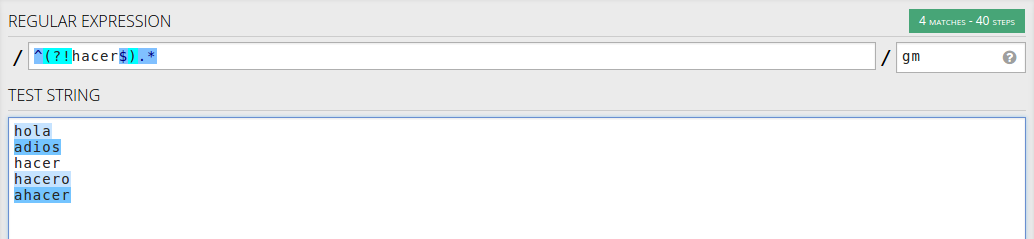
\includegraphics[width=1\linewidth]{negativelookahead}
		
		Arriba, la expresión regular con los modificadores global y multilinea.
		Abajo, el texto al que se le pasa la expresión regular. Como se puede ver, todo hace match salvo la palabra `hacer'.
	\end{center}
	
	

	
\end{document}